\chapter{Základné tipy na písanie v \LaTeX-u} \label{sec:tipy}

Úlohou tejto kapitoly nie je byť príručkou k LaTeX-u. Na internete ich nájdete kopec, výborná je napríklad \href{https://www.overleaf.com/learn}{táto príručka na stránke Overleaf-u} alebo \href{https://en.wikibooks.org/wiki/LaTeX}{táto na eikibooks}. Pri písaní určite pomôžu aj rôzne fóra, napríklad \href{https://tex.stackexchange.com/}{https://tex.stackexchange.com/}. Uvádzam len niekoľko základných tipov pre písanie matematickej záverečnej práce v LaTeX-u. Keď budete pri písaní niečo potrebovať, môžete sa inšpirovať, resp. si to odtiaľto skopírovať a upraviť.

Určite existuje veľa užitočných príkazov a balíkov, o~ktorých neviem/nepoužívam ich. Človek sa v LaTeX-u má čo učiť celý život.

\section{Vymenovanie, číslovanie}

\paragraph{Vymenovávanie cez odrážky}
\begin{itemize}
	\item Prvá odrážka
	\item Druhá odrážka
	\item Poďme o level hlbšie
	\begin{itemize}
		\item Odrážka o level hlbšie
		\item Ešte jedna 
	\end{itemize}
	\item Posledná odrážka
\end{itemize}

\paragraph{Číslovanie}
\begin{enumerate}
	\item Ovocie
	\item Zelenina
	\item Pečivo
	\begin{enumerate}
		\item Chlieb
		\item Rožky
	\end{enumerate}
\end{enumerate}

\paragraph{Abecedné číslovanie}
\begin{enumerate}[label=\alph*)]
	\item Parabolická rovnica
	\item Hyperbolická rovnica
	\item Eliptická rovnica
\end{enumerate}

\paragraph{Číslovanie rímskymi číslicami}
\begin{enumerate}[label=\roman*)]
	\item Jablko
	\item Banán
	\item Mrkva
\end{enumerate}

\paragraph{Číslovanie bez medzier medzi položkami}
\begin{enumerate}
	\setlength{\itemsep}{0pt}
	\setlength{\parskip}{0pt}
	\item Kameň
	\item Papier
	\item Nožnice
\end{enumerate}

\section{Rovnice}
Písanie rovníc je veľká téma a je to jedna z nasilnejších stránok LaTeX-u. V podstate všetko, čo vás napadne napísať, sa dá napísať, len stačí vygoogliť ako. Veľmi dobre je písanie rovníc rozobraté \href{https://www.overleaf.com/learn/latex/Mathematical_expressions}{tu na stránke Overleaf-u}, určite si to prebehnite (aj podstránky uvedené dole). Nebudem rozoberať, ako sa píšu matematické symboly, zlomky, sumy, integrály, matice,... (to si ľahko nájdete). Budem sa skôr venovať prostrediam pre tvorbu rovníc a referencovaniu rovníc, to býva väčší problém.

Na písanie rovníc sú dva režimy:
\begin{itemize}
	\item \textbf{Inline}: Vzorec je súčasťou textu. Napríklad $a^2+b^2=c^2$ alebo \(x\in\mathbb{R}\). Je viacero ekvivalentných spôsobov, ako ich písať, najčastejšie sa používa syntax \verb|$...$| alebo \verb|\(...\)|.
	\item \textbf{Display}: Vzorec je na samostatnom riadku. Napríklad
	\begin{equation*} 
		f(x)=ax^2+bx+c
	\end{equation*}
	alebo
	\[ \sin^2x=\frac{1-\cos2x}{2}, \qquad \cos^2x=\frac{1+\cos2x}{2}. \]
	Keď sa na rovnicu chceme v texte odvolať, použijeme automatické číslovanie
	\begin{equation}\label{eq:Gauss}
		\int\limits_{V} \nabla\cdot\vec{F}\,dx = \int\limits_{\partial V} \vec{F}\cdot\vec{n}\,dS.
	\end{equation}
\end{itemize}

Keď potrebujete napísať dlhú rovnicu na viac riadkov alebo viac rovníc pod seba a zarovnať ich, je na to v balíku \verb|amsmath| veľa prostredí. Neurobte tú chybu (čo som kedysi robil aj ja), že sa naučíte iba jedno -- dve a s nimi budete robiť. Pri písaní vzorcov sa vyskytnú rôzne situácie a vhod môže prísť raz jedno prostredie, raz iné. Niekedy je dobré skúsiť viac možností a zistiť, čo vyzerá lepšie. Často existuje aj viacero riešení pre dosiahnutie rovnakého výsledku. Uvediem niekoľko príkladov prostredí, ktoré by sa mohli hodiť (niektoré sú zo stránky Overleaf-u).

Prostredie \verb|align| sa používa takto
\begin{align}
	x + y  & = 1, \label{eq:align1} \\
	2x - y & = 5. \label{eq:align2}
\end{align}
Komplikovanejší príklad použitia \verb|align| je tu
\begin{align*}
	x&=y,           &  w &=z,              &  a&=b+c,\\
	2x&=-y,         &  3w&=\frac{1}{2}z,   &  a&=b,\\
	-4 + 5x&=2+y,   &  w+2&=-1+w,          &  ab&=cb.
\end{align*}
Ak máme viacero stĺpcov rovníc (ako v predchádzajúcom príklade), vhodné je aj prostredie \verb|alignat|. V ňom sa dá dobre ovládať vzdialenosť stĺpcov rovníc.
\begin{alignat*}{3}
	x       & =y,   & \hspace{1.5cm}  w  & =z,            & \hspace{1.5cm} a & =b+c, \\
	2x      & =-y,  & \hspace{1.5cm} 3w  & =\frac{1}{2}z, & \hspace{1.5cm}a  & =b,   \\
	-4 + 5x & =2+y, & \hspace{1.5cm} w+2 & =-1+w,         & \hspace{1.5cm}ab & =cb.
\end{alignat*}
Ak chcete dve rovnice, ale len jeden label, môžete použiť napríklad \verb|split| vnútri \verb|equation|
\begin{equation} \label{eq:equation_split}
	\begin{split}
		A & = \frac{\pi r^2}{2}, \\
		& = \frac{1}{2} \pi r^2.
	\end{split}
\end{equation}
Ak máme sústavu rovníc \eqref{eq:sustava}, ktorú chceme zarovnať do viacero stĺpcov a zároveň ju chceme očíslovať jedným labelom, dá sa to urobiť pomocou prostredia \verb|aligned| vnútri \verb|equation| takto
\begin{equation}\label{eq:sustava}
	\begin{aligned}
		0. \mbox{ rovnica}     & \quad & u_0                   & =0,             \\
		1. \mbox{ rovnica}     & \quad & -u_0+2u_1-u_2         & =f(x_1)h^2,     \\
		2. \mbox{ rovnica}     & \quad & -u_1+2u_2-u_3         & =f(x_2)h^2,     \\
		\vdots                 &  \\
		i. \mbox{ rovnica}     & \quad & -u_{i-1}+2u_i-u_{i+1} & =f(x_i)h^2,     \\
		\vdots                 &  \\
		(n-1). \mbox{ rovnica} & \quad & -u_{n-2}+2u_{n-1}-u_n & =f(x_{n-1})h^2, \\
		n. \mbox{ rovnica}     & \quad & u_n                   & =1.
	\end{aligned}
\end{equation}
Ak sa vám rovnica nezmestí na riadok, môžete použiť prostredie \verb|multline|
\begin{multline}
	p(x) = c_0+c_1x+c_2x^2+c_3x^3+c_4x^4+c_5x^5+c_6x^6+c_7x^7+c_8x^8\\ 
	+c_9x^9+c_{10}x^{10}+c_{11}x^{11}+c_{12}x^{12}+c_{13}x^{13}+c_{14}x^{14},
\end{multline}
ale dá sa to (inak) vyriešiť aj pomocou \verb|align|
\begin{align}
	p(x) = c_0+c_1x+c_2x^2+&c_3x^3+c_4x^4+c_5x^5+c_6x^6+c_7x^7+c_8x^8 \nonumber\\ 
	&+c_9x^9+c_{10}x^{10}+c_{11}x^{11}+c_{12}x^{12}+c_{13}x^{13}+c_{14}x^{14}. \label{eq:long_equation}
\end{align}
Záleží od situácie, čo sa viac hodí. Po častiach definovaná funkcia sa robí pomocou prostredia \verb|cases| takto
\begin{equation*}
	w(x)=
	\begin{cases}
		(x-x_1)^2(x-x_2)^2,& x\in[x_1,x_2],\\
		0,& \mbox{inak}.
	\end{cases}
\end{equation*}
Prostredie \verb|aligned| vnútri \verb|equation| sa hodí napríklad v tejto situácii
\begin{equation}
	\begin{aligned}
		a + b x_1^e&=u_1^e\\
		a + b x_2^e&= u_2^e
	\end{aligned}
	\hskip 1cm \mbox{resp. maticovo} \hskip 1cm 
	\begin{bmatrix}
		1 & x_1^e \\ 
		1 & x_2^e
	\end{bmatrix}
	\begin{bmatrix}
		a  \\ 
		b 
	\end{bmatrix}=
	\begin{bmatrix}
		u_1^e  \\ 
		u_2^e 
	\end{bmatrix}.
\end{equation}
Niekedy pri zarovnávaní môže byť vhodné použiť aj prostredie \verb|array|
\begin{align*}
	\begin{array}{lrl}
		\text{\multirow{2}{*}{$\Omega^{e-1}:$}} & K_{11}^{e-1} u_1^{e-1} + K_{12}^{e-1} u_2^{e-1} & = f_1^{e-1} + Q_1^{e-1}, \\
		& \color{Green} K_{21}^{e-1} u_1^{e-1} + K_{22}^{e-1} u_2^{e-1} & \color{Green}= f_2^{e-1} + \underline{Q_2^{e-1}}, \\
		\text{\multirow{2}{*}{$\Omega^e:$}} & \color{Green}K_{11}^e u_1^e + K_{12}^e u_2^e & \color{Green}= f_1^e + \underline{Q_1^e}, \\
		& K_{21}^e u_1^e + K_{22}^e u_2^e & = f_2^e + Q_2^e.
	\end{array}
\end{align*}
Kvôli ľahšiemu referencovaniu sa občas môže hodiť aj prostredie \verb|subequations|. Maxwellove rovnice majú tvar
\begin{subequations}
	\label{eq:Maxwell}
	\begin{align}
		\nabla\cdot\mathbf{D}  & =\rho,    \label{eq:Maxwell_1}                                               \\
		\nabla\times\mathbf{E} & = -\frac{\partial \mathbf{B}}{\partial t},  \label{eq:Maxwell_2}             \\
		\nabla\cdot\mathbf{B}  & =0,    \label{eq:Maxwell_3}                                                  \\
		\nabla\times\mathbf{H} & = \frac{\partial \mathbf{D}}{\partial t} + \mathbf{J}.  \label{eq:Maxwell_4}
	\end{align}
\end{subequations}
Môžeme sa potom na ne odvolávať naraz \eqref{eq:Maxwell} alebo aj jednotlivo \eqref{eq:Maxwell_2}.


\begin{rem}
	Existuje ešte aj prostredie \verb|eqnarray|, ale \href{https://tex.stackexchange.com/questions/196/eqnarray-vs-align}{nepoužívajte ho, môžu s ním byť problémy}.
\end{rem}

\begin{rem}[Vzorcová interpunkcia]
	V slovenčine by sa mala používať vzorcová interpunkcia -- aj vzorec v režime display je súčasťou vety, a preto by sa mala používať interpunkcia (čiarky, resp. bodky) podobne, akoby rovnica bola v režime inline, pozri napríklad rovnice \eqref{eq:align1} a \eqref{eq:align2}. Sú prípady, kedy interpunkcia môže byť vizuálne rušivá,\footnote{Čo je rušivé a čo nie, je otázka vkusu. Vkus sa aj časom mení, ja som napríklad kedysi vzorcovú interpunkciu nepoužíval vôbec.} vtedy jej použitie treba zvážiť.
\end{rem}



\subsection{Fyzikálne jednotky}
Na písanie fyzikálnych jednotiek je vhodný balík \verb|siunitx|. Základné použitie vyzerá takto
\begin{itemize}
	\item Jednotka zrýchlenia je $\si{kg.m.s^{-2}}$.
	\item Gravitačné zrýchlenie má hodnotu $g=\SI{9,8}{kg.m/s^2}$.
	\item Youngov modul pružnosti ocele je $E=\SI{200}{GPa}=\SI{2e11}{Pa}$.
	\item Pravý uhol je $\pi/2=\ang{90}$, štvrtina z neho je $\pi/8=\ang{22.5}=\ang{22;30;}$.	
\end{itemize}
Ďalšie možnosti nájdete v dokumentácii balíka \verb|siunitx| (v TeXstudiu \verb|Ctrl|+klik na \verb|siunitx| v preambule v riadku \verb|\usepackage{siunitx}|).


\section{Definície, vety, dôkazy}
V niektorých prácach môže byť vhodné používanie štýlu \uv{Definícia-Veta-Dôkaz} (prípadne aj Lemma, Poznámka, Príklad,...). V preambule sú kvôli tomu riadky:
\begin{verbatim}
	% Definície, Vety, Dôkazy...
	\usepackage{amsthm}
	\theoremstyle{definition}
	\newtheorem{thm}{Veta}[section]
	\newtheorem{defn}[thm]{Definícia}
	\newtheorem{lem}[thm]{Lemma}
	\newtheorem{cor}[thm]{Dôsledok}
	\newtheorem{rem}[thm]{Poznámka}
	\newtheorem{exmp}[thm]{Príklad}
\end{verbatim}
Nastavenie a spôsob číslovania jednotlivých prostredí si v týchto riadkoch môžete podľa potreby upraviť, viac sa dozviete napríklad \href{https://www.overleaf.com/learn/latex/Theorems_and_proofs}{na tejto stránke}.

Použitie vyzerá takto:

\begin{defn}[Slabé riešenie]\label{def:SlabeRies}
	Nech funkcia $f$ je z priestoru $L_2(0,1)$. \textbf{Slabým riešením} okrajovej úlohy~\eqref{} nazývame funkciu $u$ z priestoru $V$ takú, že pre všetky váhové funkcie $w\in V$ platí
	\begin{equation*}
		(u,w)_A=(f,w).
	\end{equation*}
\end{defn}
\begin{thm}[Vlastnosť ortogonality]
	Chyba  $\varepsilon=U-u$ je v zmysle energetického skalárneho súčinu kolmá (ortogonálna) na všetky funkcie $w\in S \subset V$, teda
	\begin{equation}\label{eq:Ortogonalita}
		(\varepsilon,w)_A=(U-u,w)_A=0.
	\end{equation}
\end{thm}
\begin{proof}
	Pre približné riešenie $U$ platí rovnica
	\begin{equation}\label{eq:RG2}
		(U,w)_A=(f,w),\qquad \mbox{pre všetky } w \in S\subset V.
	\end{equation}
	Podobne pre slabé riešenie $u$ podľa Definície~\ref{def:SlabeRies} platí
	\begin{equation}\label{eq:SlabeRies2}
		(u,w)_A=(f,w),\qquad \mbox{pre všetky } w \in V \mbox{ a teda aj pre všetky } w \in S\subset V.
	\end{equation}
	Keď rovnice~\eqref{eq:RG2} a~\eqref{eq:SlabeRies2} od seba odčítame, dostaneme vlastnosť ortogonality~\eqref{eq:Ortogonalita}.
\end{proof}


\section{Referencie a citácie}
Na orientáciu v práci slúžia referencie. Môžu odkazovať na všeličo, len to musí byť označené pomocou \verb|\label{name}|. Reťazec \verb|name| by mal byť výstižný (nie len nejaké číslo), v zdrojovom kóde je to potom prehľadnejšie a lepšie sa s labelami pracuje. Je vhodné si v labelovaní zaviesť nejakú konvenciu. Štandardne sa používa pre obrázky \verb|\label{fig:name}|, pre rovnice \verb|\label{eq:name}|, pre časti a kapitoly \verb|\label{sec:name}| a podobne. Takáto konvencia je výhodná napríklad aj keď máte sekciu, obrázok a rovnicu, ktoré hovoria o jednej veci, tak to ľahko odlíšite. Reťazec \verb|name| môže obsahovať aj medzery, ale používajte radšej podčiarkovník. Uvediem niekoľko príkladov referencií.
\begin{description}
	\item[Kapitola, sekcia.] V kapitole~\ref{sec:aky_editor} sme hovorili o tom, aký editor použiť. V časti~\ref{sec:sekcia} sme len bľabotali.
	\item[Obrázok, tabuľka.] Pozri Obrázok~\ref{fig:bod_v_rovine}. Tabuľka~\ref{tab:resultsDDFV} je tiež pekná.
	\item[Rovnica.] Vzťah~\eqref{eq:Gauss} je Gaussova veta. Na referencovanie rovníc je efektívnejšie (rýchlejšie) používať \verb|\eqref{label}|, nie \verb|(\ref{label})|.
	\item[Strana.] Občas sa zíde referencia na stranu. Na strane \pageref{sec:clenenie} sme hovorili o členení práce.
\end{description}

V záverečnej práci je veľmi dôležité poriadne citovať zdroje. Najefektívnejšie je používať balík \verb|biblatex|. Často sa stretávam s tým, že ľudia vypisujú bibliografiu \uv{natvrdo} manuálne. Nerobte túto chybu. Všetky zdroje treba dať do súboru \verb|.bib|, ktorý je databázou vašich zdrojov. Balík \verb|biblatex| sa postará o správne formátovanie a zoradenie položiek v bibliografii.

Ako do bibliografickej databázy v súbore \verb|.bib| efektívne pridávať nové položky? Veľa z nich nájdete na internete v rôznych databázach publikácií a na stránkach vedeckých časopisov. Ručné vpisovanie bibliografických údajov by malo byť až poslednou voľbou.
\begin{itemize}
	\item Odkazy na vedecké články a knihy väčšinou nájdete na pár klikov na \url{https://scholar.google.com/}. Ak chcete pridať odkaz napríklad na vedecký článok~\cite{mikulaRemesikovaSarkoci2014}, stačí po vyhľadaní kliknúť na \uv{Citovať} (Obr.~\ref{fig:google_scholar}) a zvolíte BiBTeX.
	\item Ak chcete pridať odkaz na vedecký článok, napríklad~\cite{mikulaRemesikovaSarkoci2014}, položku do databázy s veľkou pravdepodobnosťou nájdete aj cez \href{https://www.researchgate.net/publication/275063142_Manifold_Evolution_with_Tangential_Redistribution_of_Points}{www.researchgate.net}, klik na Download citation. Položku štandardne nájdete aj na \href{https://epubs.siam.org/doi/10.1137/130927668}{stránke časopisu}, v ktorom článok vyšiel. Vždy treba hľadať niečo v zmysle \uv{download citation}, \uv{cite this paper} a podobne, a následne zvoliť BiBTeX.
\end{itemize}

Na položky z bibliografickej databázy potom v texte odkazujete. Môžete citovať jednu položku~\cite{eymard}, alebo aj viacero naraz~\cite{Handlovicova,mikulaRemesikovaSarkoci2014}.

\begin{figure}[h]
	\centering
	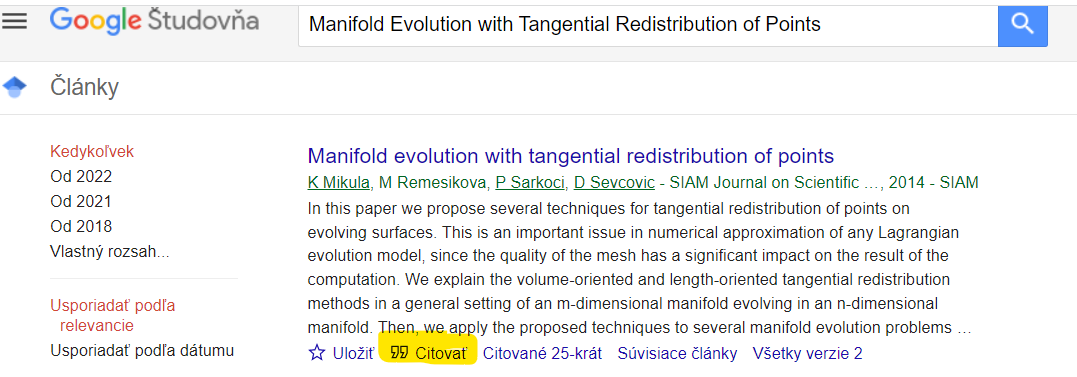
\includegraphics[width=1.0\linewidth]{google_scholar}
	\caption{Google scholar.}
	\label{fig:google_scholar}
\end{figure} 


\section{Obrázky}
Obrázky sú veľmi dôležitý prvok záverečnej práce. Keď sú dobre urobené, môžu čitateľovi veľmi pomôcť prácu pochopiť. Je veľa možností, ako obrázky vkladať do TeX-u a ešte viac možností, ako ich vytvárať. Obrázky, ktoré chcete vložiť do práce je dobré mať pokope v priečinku/pričinkoch. V preambule je cesta k priečinku nastavená pomocou príkazu \verb|\graphicspath{ {./figures/} }|.

\subsection{Vkladanie obrázkov}\label{sec:vkladanie_obrazkov}

\subsubsection{Jeden obrázok}
O tom, ako vkladať obrázky do TeX-u sa prehľadne píše napríklad \href{https://www.overleaf.com/learn/latex/Inserting_Images}{tu na stránke Overleaf-u} alebo \href{https://en.wikibooks.org/wiki/LaTeX/Importing_Graphics}{na wikibooks tu} a \href{https://en.wikibooks.org/wiki/LaTeX/Floats,_Figures_and_Captions}{tu}. Jednoduché vloženie obrázka sa robí takto:

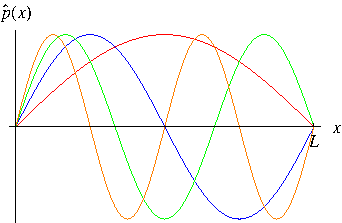
\includegraphics[width=0.35\textwidth]{stoj2}

Takýto obrázok ale nie je vycentrovaný a nemá popis. V práci by mali mať všetky obrázky číslo a popis, potom sa na ne ľahko odvolávalo v texte. Takýmto príkladom je Obrázok~\ref{fig:klavir}.\footnote{Všimnite si, že v zdrojovom kóde je (zakomentovaný) \textbackslash vspace\{...\}, pomocou ktorého môžete zväčšiť/zmenšiť biele miesto pod/nad obrázkom a pod popisom, to sa občas môže hodiť.}

\begin{figure}[h]
	\centering
	%\vspace{-5pt}
	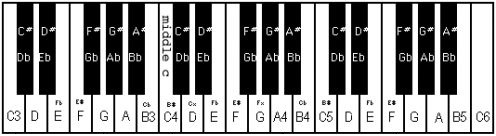
\includegraphics[width=0.6\textwidth]{klavir2}
	%\vspace{-10pt}
	\caption{Označenia tónov na klaviatúre.}
	\label{fig:klavir}
	%\vspace{-5pt}
\end{figure}

\begin{wrapfigure}{r}{0.2\textwidth}
	\centering
	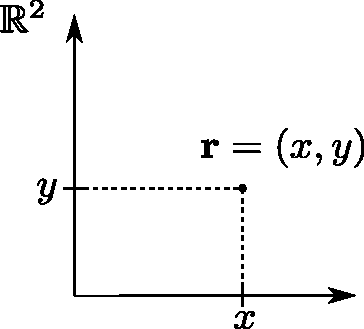
\includegraphics[width=0.2\textwidth]{bod_v_rovine}
	\caption{Inkscape.}
	\label{fig:bod_v_rovine}
\end{wrapfigure}
V TeXstudiu sa takto formátované obrázky dajú do kódu vkladať veľmi jednoducho pomocou \verb|Ctrl+C| -- \verb|Ctrl+V|, resp. drag and drop. Funguje to aj so screenshotmi,\footnote{Mimochodom, poznáte klávesovú skratku Windows+Shift+S? Nie? Tak skúste, odpadnete z nej :-).} po vložení do TeXstudia sa zobrazí okno, v ktorom screenshot uložíte do priečinka s obrázkami.

Obrázky~\ref{fig:bod_v_rovine},~\ref{fig:parabola} obtekané textom sa vkladajú pomocou balíka \verb|wrapfig|.

\textit{Lorem ipsum dolor sit amet, consectetur adipiscing elit. Cras mollis metus metus. Nam eget sapien elementum, pharetra arcu ut, congue tortor. Nulla non tortor ullamcorper, pretium turpis ac, accumsan erat. Vestibulum porttitor leo in arcu laoreet, vitae ullamcorper massa blandit. Vestibulum fermentum euismod dui, vel blandit dolor. Maecenas aliquam pharetra nunc, quis mollis turpis sodales non. Nunc non odio condimentum, sollicitudin diam sit amet, vestibulum libero. Ut sed euismod leo. Cras pharetra dolor metus, vitae auctor ligula porttitor ut. Vestibulum eu risus non velit egestas pulvinar. Nam feugiat sed libero eget consequat. Proin ligula turpis, facilisis et nisi in, vehicula fringilla libero. Nulla sagittis velit odio, in faucibus est vulputate non.}

\begin{wrapfigure}{l}{0.25\textwidth}
	\centering
	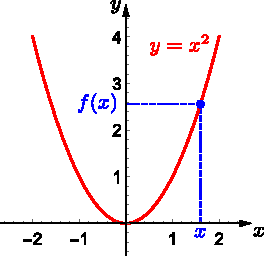
\includegraphics[width=0.25\textwidth]{parabola}
	\caption{Mathematica+Inkscape.}
	\label{fig:parabola}
\end{wrapfigure}
\textit{Suspendisse tempor dictum mollis. Quisque ac ante arcu. Class aptent taciti sociosqu ad litora torquent per conubia nostra, per inceptos himenaeos. Pellentesque tincidunt consequat faucibus. Nullam vel iaculis nisl. Quisque viverra sed dui fermentum congue. Nullam venenatis, mi eget pulvinar condimentum, quam massa euismod lacus, quis pulvinar neque lacus vestibulum arcu. Maecenas porta lobortis nibh. Orci varius natoque penatibus et magnis dis parturient montes, nascetur ridiculus mus. Quisque id semper lorem, nec aliquet odio. Nulla ornare consectetur odio ullamcorper auctor. Sed lobortis nisl vitae mauris porttitor facilisis. Nullam neque quam, finibus at tortor et, maximus ultrices magna. Duis ultricies malesuada lacus, ut gravida ante tempus eu.}

\textit{Vestibulum tortor diam, lacinia porttitor tincidunt nec, suscipit ac mi. Sed in nunc a tellus egestas porta. Vivamus at metus condimentum, laoreet nisl vel, fringilla ante. Nunc quis libero a felis tempus imperdiet sit amet sed mauris. Sed justo sem, laoreet eu accumsan a, tincidunt sit amet felis. Duis at pharetra libero. Sed et ligula urna. Integer pulvinar pellentesque velit, sit amet vulputate tortor. Curabitur ultrices rutrum enim et suscipit. Nam dictum vestibulum odio eu malesuada.}


\subsubsection{Viac obrázkov}

Príklad dvoch obrázkov vložených vedľa seba vidíme na Obrázku~\ref{fig:hyperbolicky_paraboloid}. Analogicky sa dajú urobiť aj 3 obrázky vedľa seba, prípadne mriežka obrázkov (napr. 4x2, ako vidíme na Obrázku~\ref{fig:bumpy_sphere}). Niekedy, keď je v práci veľmi veľa obrázkov, môže byť vhodné vytvoriť strany, na ktorých sú len obrázky, príkladom je Obrázok~\ref{fig:bumpy_sphere}.
\begin{figure}[h!]
	\centering
	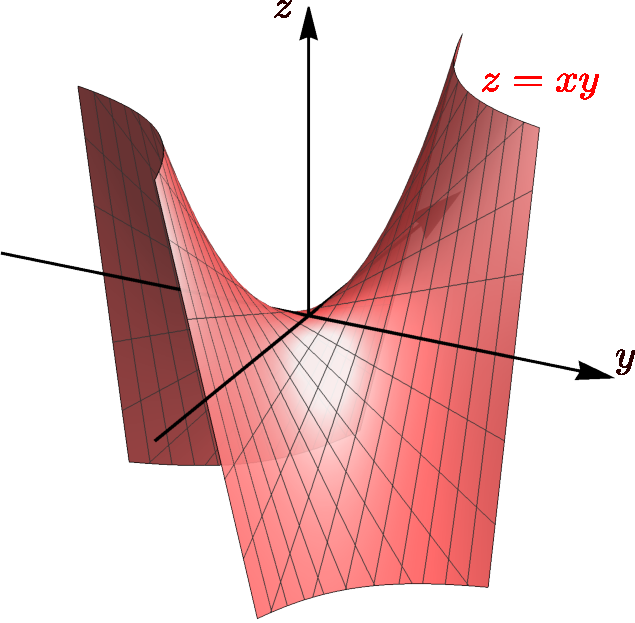
\includegraphics[height=5cm]{fig_hyperbolicky_paraboloid}
	\quad
	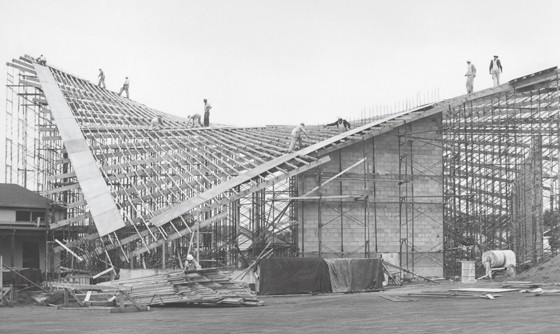
\includegraphics[height=5cm]{st_chas_framing}
	\caption{Graf funkcie $f(x,y)=xy$ a konštruovanie strechy v tvare hyperbolického paraboloidu (v menšom okolí sedlového bodu, než vykresľujeme v grafe).} \label{fig:hyperbolicky_paraboloid}
\end{figure}
Ak ale chceme, aby každý obrázok mal svoje číslo a popis, môžeme to urobiť napríklad tak, ako vidíme na príklade Obrázkov~\ref{fig:vzduchovod_geom}~a~\ref{fig:vzduchovod_mesh}.
\begin{figure}[!h]
	\centering
	\vspace{-5pt}
	\begin{minipage}{.5\textwidth}
		\centering
		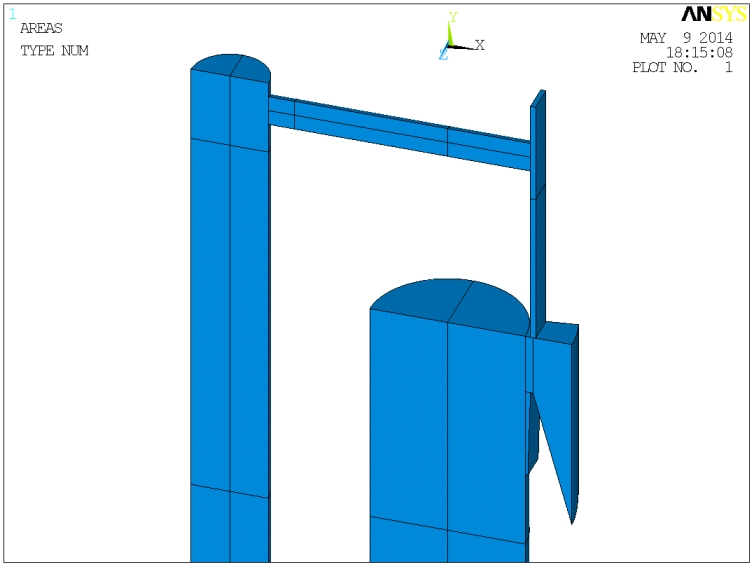
\includegraphics[width=0.95\textwidth]{vzduchovod1}
		\vspace{-5pt}
		\caption{Obrázok z ANSYS-u.}
		\label{fig:vzduchovod_geom}
	\end{minipage}%
	\begin{minipage}{.5\textwidth}
		\centering
		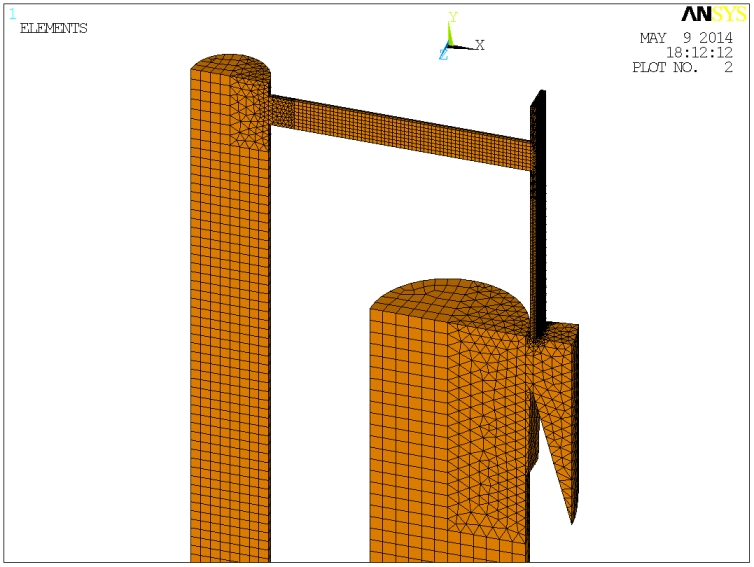
\includegraphics[width=0.95\textwidth]{vzduchovod2}
		\vspace{-5pt}
		\caption{Obrázok z ANSYS-u.}
		\label{fig:vzduchovod_mesh}
	\end{minipage}
	\vspace{-5pt}
\end{figure}

Pomocou balíka \verb|subcaption| sa dajú podobne vložiť vedľa seba tak, ako vidíme na Obrázku~\ref{fig:matlab}, pričom môžu mať jeden hlavný popis a ďalšie podpopisy \ref{fig:matlab_2D}~resp.~\ref{fig:matlab_3D}.
\begin{figure}[h!]
	\centering
	\begin{subfigure}[b]{0.45\textwidth}
		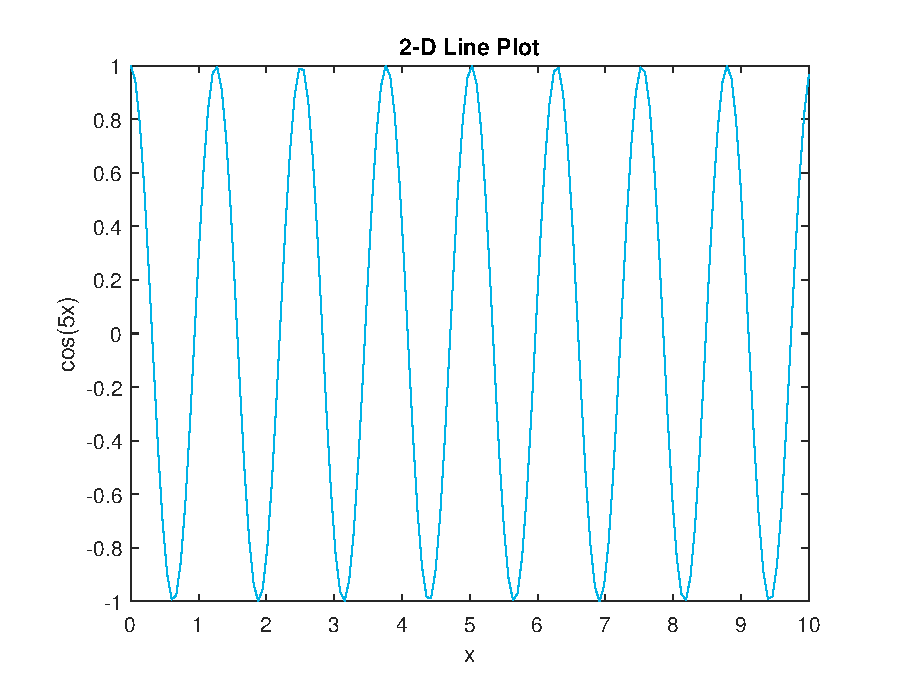
\includegraphics[width=\textwidth]{matlab_2D}
		\caption{Graf funkcie jednej premennej (2D).}
		\label{fig:matlab_2D}
	\end{subfigure}
	\qquad
	\begin{subfigure}[b]{0.45\textwidth}
		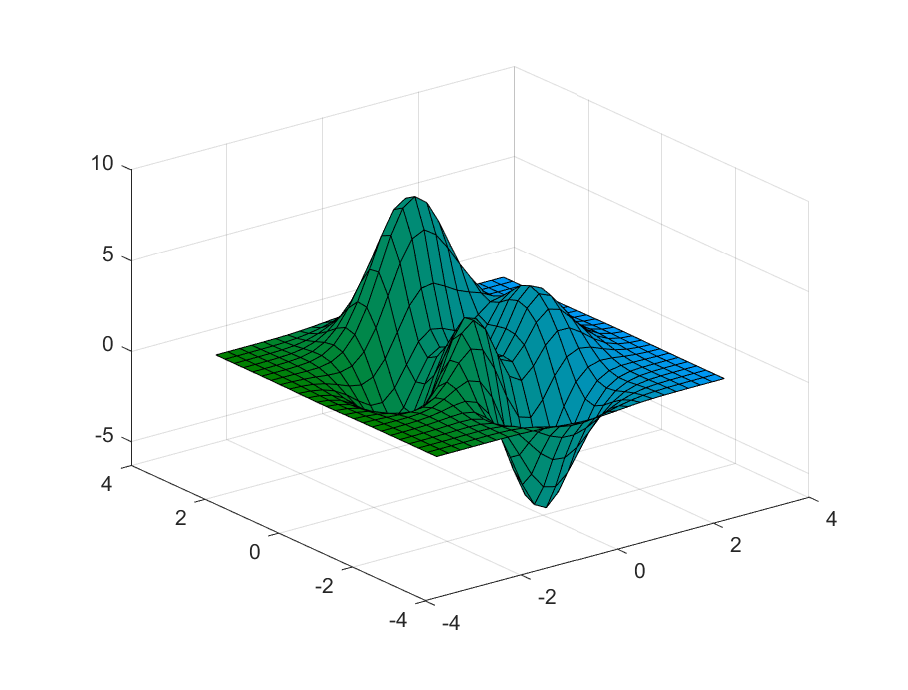
\includegraphics[width=\textwidth]{matlab_3D}
		\caption{Graf funkcie v dvoch premenných (3D).}
		\label{fig:matlab_3D}
	\end{subfigure}
	\caption{Príklady obrázkov z MATLAB-u.}\label{fig:matlab}
\end{figure}

\begin{figure}[p]
	%	\vspace{-5pt}
	\centering
	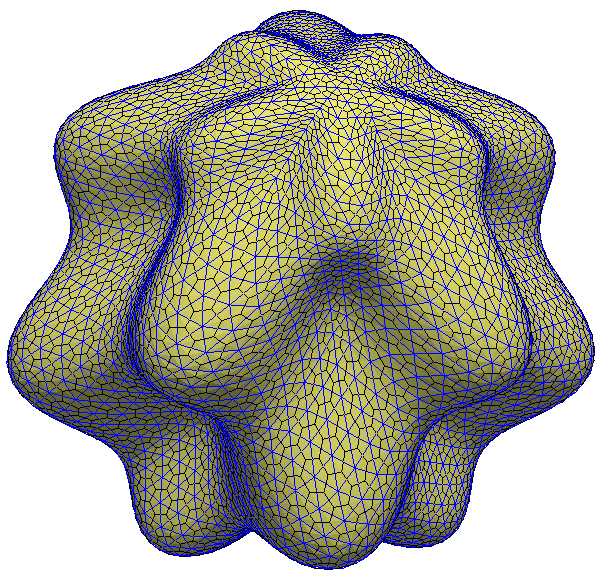
\includegraphics[width=0.35\textwidth]{bumpy_noRed_level5_tstep0_FT.png}
	\hspace{0.1\textwidth}
	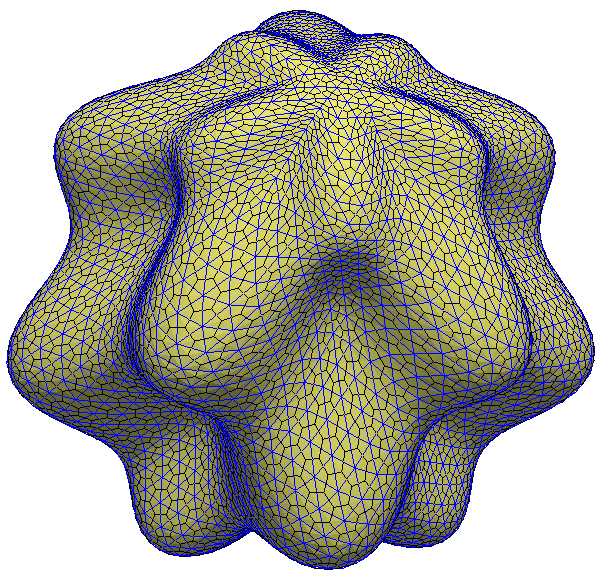
\includegraphics[width=0.35\textwidth]{bumpy_noRed_level5_tstep0_FT.png}
	\newline
	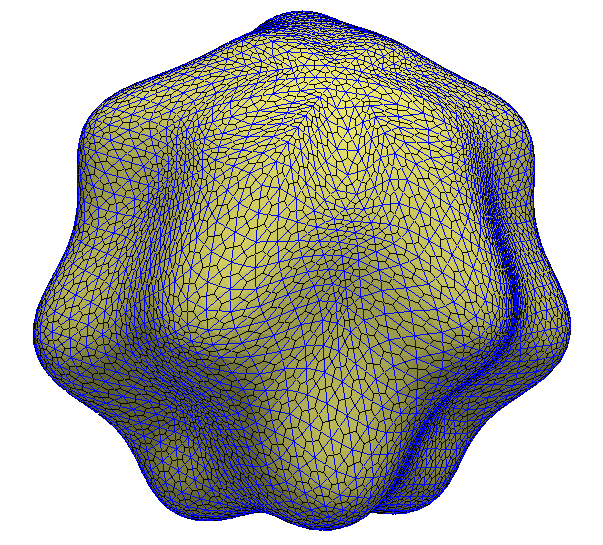
\includegraphics[width=0.35\textwidth]{bumpy_noRed_level5_tstep20.png}
	\hspace{0.1\textwidth}
	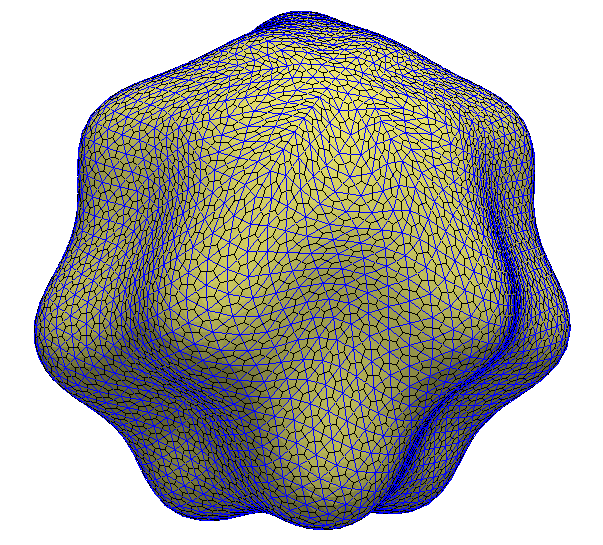
\includegraphics[width=0.35\textwidth]{bumpy_omega100_level5_tstep20.png}
	\newline
	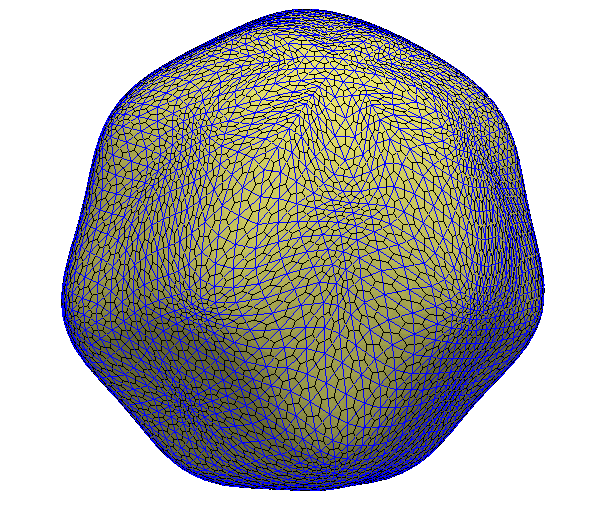
\includegraphics[width=0.35\textwidth]{bumpy_noRed_level5_tstep50.png}
	\hspace{0.1\textwidth}
	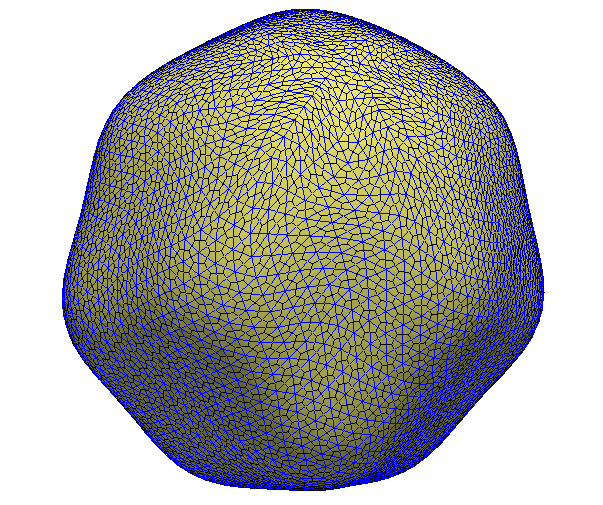
\includegraphics[width=0.35\textwidth]{bumpy_omega100_level5_tstep50.png}
	\newline
	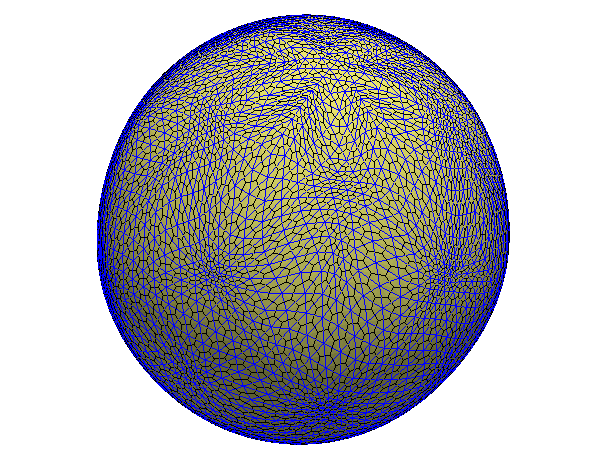
\includegraphics[width=0.35\textwidth]{bumpy_noRed_level5_tstep128.png}
	\hspace{0.1\textwidth}
	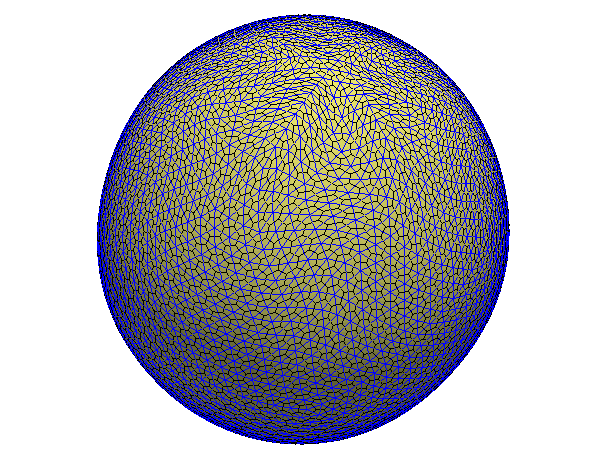
\includegraphics[width=0.35\textwidth]{bumpy_omega100_level5_tstep128.png}
	\newline
	%	\vspace{-5pt}
	\caption{Príklady obrázkov z ParaView.}\label{fig:bumpy_sphere} 
	%\vspace{-10pt}
\end{figure}

\subsection{Vytváranie obrázkov}

Z časti \ref{sec:vkladanie_obrazkov} už máme predstavu, ako vkladať existujúce obrázky (resp. výstupné obrázky zo softvéru, napríklad z ANSYS-u). V akom programe ale vytvárať nové grafy a obrázky? Toto je (prekvapujúco?) ťažká otázka.

\paragraph{Aké formáty používať?}

\begin{itemize}
	\item \textbf{Vektorová grafika:} PDF, EPS (LaTeX ale aj tak EPS skonvertuje na PDF).
	\item \textbf{Rastrová grafika:} PNG, JPG (odporúčam radšej PNG, lebo pri ukladaní do JPG resp. JPEG sa kvôli kompresii znižuje kvalita a vzniká šum).
\end{itemize}
Kvôli kvalite obrázkov \textbf{preferujte vektorovú grafiku} (ak je to možné). V elektronickej verzii práce sú vektorové obrázky aj po priblížení stále pekné, hladké. Pri grafike, ktorá je tieňovaná (napr. vrstevnicové grafy, plochy v 3D) je lepšie obrázok v dostatočnej kvalite uložiť ako raster. Vo všeobecnosti je dobré obrázky ukladať tak, aby boli orezané, bez veľkého nadbytočného orámovania okolo toho, čo nás zaujíma.


\paragraph{Mathematica.}

V softvéri Mathematica robiť viete, preto je dobrý nápad tvoriť grafy/obrázky v ňom. Pre export nepoužívajte screenshot, ale export:
\begin{itemize}
	\item \textbf{2D grafika:} \verb|pravý klik na obrázok/Save Graphic As/pdf|. Grafika bude automaticky vektorová.
	\item \textbf{3D grafika:} \verb|pravý klik na obrázok/Save Graphic As/png| (obrázok treba mať pred uložením dostatočne veľký). Je dobré ešte pred uložením obrázka odstrániť Bounding Box: \verb|pravý klik na| \verb|obrázok/| \verb|Trim| \verb|Bounding Box|, aby okolo obrázka nebolo zbytočne veľa bielej plochy.
\end{itemize}
Obrázok sa dá uložiť aj pomocou príkazu \verb|Export| (zíde sa napríklad vtedy, keď potrebujete export automatizovať počas behu kódu alebo si ukladanie zautomatizovať).


\paragraph{MATLAB.}

Ak viete robiť MATLAB-e, prípadne v ňom programujete program k záverečnej práci, je dobrý nápad robiť grafy/obrázky v ňom. Pre export nepoužívajte screenshot, ale export v okne Figure:
\begin{itemize}
	\item \textbf{2D grafika:} \verb|klik na File/Save As/eps|.\footnote{PDF tu nefunguje dobre, vloží obrázok do stredu A4.} Príkladom je Obrázok~\ref{fig:matlab_2D}.
	\item \textbf{3D grafika:} \verb|klik na File/Save As/png|. Príkladom je Obrázok~\ref{fig:matlab_3D}.
\end{itemize}
Je praktické si obrázky ukladať aj vo formáte .fig, aby ste ľahko mohli aj neskôr editovať rôzne nastavenia. Obrázok sa dá uložiť aj pomocou príkazu \verb|print|, v ktorom si nastavíte aj formát.


\paragraph{ParaView.}

Ak sú vaše dáta, resp. výsledky vhodné na vizualizáciu v ParaView, tak obrázky odtiaľ môžete ľahko exportovať. Platia podobné odporúčania, ako pri Mathematice a MATLAB-e. Ja tu pre všetky obrázky používam \verb|File/Save Screenshot/PNG| (alebo aj cez ikonu fotoaparátu na lište nad oknom \verb|RenderView|). V okne \verb|Save Screenshot Options| je potom vhodné nastaviť si v \verb|Coloring| pozadie na \verb|Transparent Bacground| alebo \verb|White Bacground|. Pred exportom je vhodné vypnúť \verb|Show Orientation| \verb|Axes| a nastaviť okno tak, aby nebolo príliš veľa pozadia. 
Viac sa o exportovaní obrázkov píše \href{https://docs.paraview.org/en/v5.8/UsersGuide/savingResults.html}{tu na stránke ParaView}. V ParaView boli vytvorené Obrázky~\ref{fig:bumpy_sphere}.


\paragraph{Inkscape.}

\href{https://inkscape.org/}{Inkscape} je výborný program na vytváranie vektorovej grafiky. Zíde sa, keď potrebujete kresliť schematické obrázky (nie grafy funkcií). Pracuje s formátom SVG, ale môžete importovať/exportovať do mnohých formátov (aj PDF a EPS). Veľmi odporúčam doinštalovať \href{https://inkscape.org/~jcwinkler/%E2%98%85textext}{TexText extension}, aby ste do obrázkov mohli vpisovať LaTeX-ovské symboly a vzorce. Inkscape má \href{https://inkscape.org/learn/}{výborné tutorialy} (zrejme stačia Basic+Advanced), takže sa dá celkom rýchlo zvládnuť. V Inkscape bol vytvorený napríklad obrázok~\ref{fig:bod_v_rovine}. Keď už máte niečo nakreslené, export sa urobí takto:
	\begin{enumerate}
		\item Označíte si, čo chcete exportovať.
		\item \verb|Ctrl+Shift+R| alebo \verb|Edit/Resize Page to Selection|.
		\item \verb|Ctrl+Shift+S| alebo \verb|File/Save As| a vybrať PDF. 
	\end{enumerate}
	
	\paragraph{Mathmeatica/Matlab/ParaView + Inkscape}
	
	Ak do obrázka potrebujete doplniť popisky alebo vzorce, ktoré nedokážete dobre urobiť v Mathematice (resp. inom softvéri), často je praktickejšie na to použiť vhodný editor -- napríklad Inkscape. Takouto kombinovanou technikou (Mathematica+Inkscape) bol vytvorený Obrázok~\ref{fig:rezy} (po pribížení zistíte, čo bolo dorobené v Inkscape).
	\begin{figure}[h]
		%\vspace{-10pt}
		\centering
		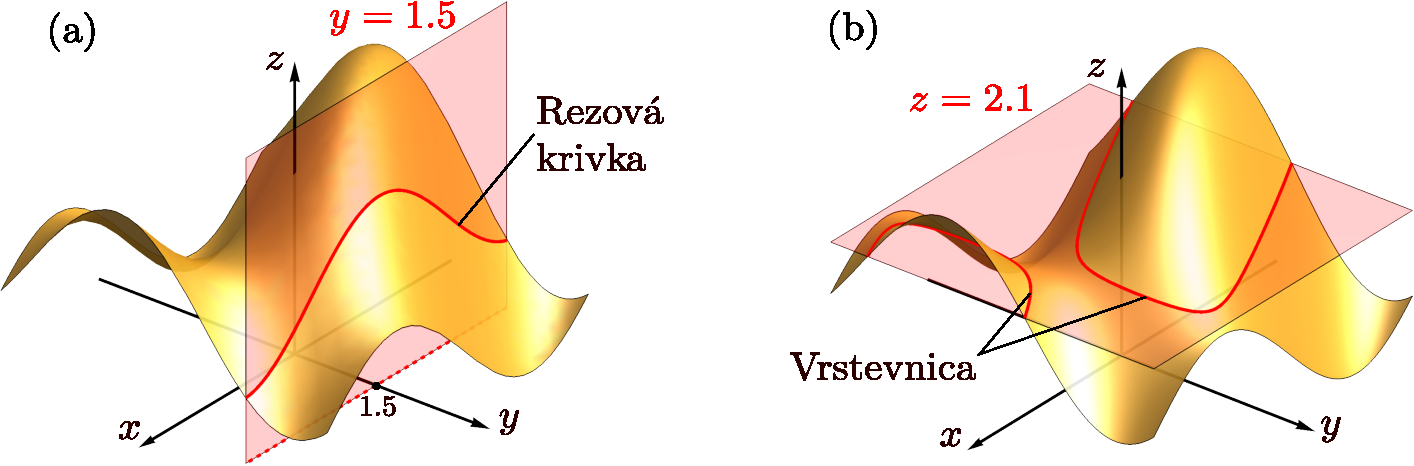
\includegraphics[width=0.8\textwidth]{fig_rezy}
		%\vspace{-10pt}
		\caption{Mathematica + dorobenie v Inkscape.} \label{fig:rezy}
		%\vspace{-5pt}
	\end{figure}
	
	
	\paragraph{Programovanie obrázkov v LaTeX-u.}
	
	Kvalitné obrázky sa dajú naprogramovať aj priamo v LaTeX-u. Nepoužívam to, ale sú ľudia, čo na tom frčia. Tu je niekoľko odkazov na túto možnosť:
	\begin{itemize}
		\item \href{https://www.overleaf.com/learn/latex/TikZ_package}{Balík TikZ} je asi najlepší. \href{https://texample.net/tikz/examples/}{Na tejto stránke} nájdete veľké množstvo príkladov -- pre predstavu, čo všetko a ako sa dá nakresliť.
		\item \href{https://en.wikibooks.org/wiki/LaTeX/Picture}{Prostredie picture}, príkladom je Obrázok~\ref{fig:picture_test}.
		\item \href{https://en.wikipedia.org/wiki/PSTricks}{Balík PSTricks}
	\end{itemize}
	Z niektorých programov na kreslenie obrázkov sa dá TeX-ovský kód generujúci obrázok exportovať (napríklad Inkscape $\rightarrow$ PStricks).
	\begin{figure}[!h]
		\centering
		\setlength{\unitlength}{0.8cm}
		\begin{picture}(6,5)
			\thicklines
			\put(1,0.5){\line(2,1){3}}
			\put(4,2){\line(-2,1){2}}
			\put(2,3){\line(-2,-5){1}}
			\put(0.7,0.3){$A$}
			\put(4.05,1.9){$B$}
			\put(1.7,2.95){$C$}
			\put(3.1,2.5){$a$}
			\put(1.3,1.7){$b$}
			\put(2.5,1.05){$c$}
			\put(0.3,4){$F=\sqrt{s(s-a)(s-b)(s-c)}$}
			\put(3.5,0.4){$\displaystyle s:=\frac{a+b+c}{2}$}
		\end{picture}
		\caption{Obrázok vytvorený pomocou prostredia picture.}
		\label{fig:picture_test}
	\end{figure}
	
	
	\section{Tabuľky}
	
	Jednoduchá tabuľka bez popisu sa robí takto:
	
	\begin{tabular}{|r|r|r|}
		\hline
		2 &   4 & 4.5 \\
		\hline
		3 &   1 &   5 \\
		18 & 4.5 &   5 \\
		\hline
	\end{tabular}
	
	Tabuľky v záverečnej práci by ale mali mať popis, tu je príklad s popisom: 
	\begin{table}[!h]
		\centering
		\caption{The $L^2$ EOC for the case with no redistribution.}
		\begin{tabular}{rlrrr}
			\hline
			$n_V$ & $\tau$     & $N$ & $ L^2\mbox{ error}$ &  EOC \\ \hline
			122 & 0.04       &   2 &            1.43e-02 &      \\
			482 & 0.01       &   8 &            3.35e-03 & 2.10 \\
			1922 & 0.0025     &  32 &            8.07e-04 & 2.05 \\
			7682 & 0.000625   & 128 &            1.95e-04 & 2.05 \\
			30722 & 0.00015625 & 512 &            4.64e-05 & 2.07 \\ \hline
		\end{tabular}
		\label{tab:resultsDDFV}
	\end{table}
	
	Ešte jeden príklad s použitím farby a definovaním šírky stĺpcov je v Tabuľke~\ref{tab:Veliciny}. Viac o tabuľkách nájdete aj s peknými príkladmi a zdrojovými kódmi \href{https://en.wikibooks.org/wiki/LaTeX/Tables#Basic_examples}{napríklad tu na wikibooks}.
	\begin{table}[h]
		\centering
		\caption{Prehľad veličín.} \label{tab:Veliciny}
		\begin{tabular}{|l|l|p{45mm}|p{60mm}|}
			\hline
			\rowcolor[gray]{.8}
			Veličina & Jednotka & Názov & Popis  \\ \hline
			$u(x,t)$ & $\si{K}$ & Teplota v~mieste $x$ a čase $t$ &   \\ \hline
			$c(x)$ & $\si{J/kg.K}$ & Merná tepelná kapacita & Množstvo tepla (J) potrebné na zohriatie 1 kg látky o 1 K  \\ \hline
			$\rho(x)$ & $\si{kg/m^3}$ & Hustota &  \\ \hline
			$f(x,t)$ & $\si{J/m^3}$s & Intenzita (hustota) \newline zdrojov tepla & Množstvo tepla (J) vyprodukované v~$\SI{1}{m^3}$ za 1 s   \\ \hline
			$q(x,t)$ & $\si{J/m^2.s}$ & Hustota tepelného toku & Množstvo tepla, ktoré prejde prierezom $\SI{1}{m^2}$ za 1 s  \\ \hline
			$\lambda(x)$ & $\si{W/m.K}$ & Koeficient (súčiniteľ)\newline tepelnej vodivosti & Množstvo tepla, ktoré prejde za 1 s medzi protiľahlými stenami jednotkovej kocky, keď sa ich teploty líšia o 1 K a ostatné steny sú izolované. \\ \hline
		\end{tabular}
	\end{table}
	
	\paragraph{Dôležitý tip.}
	Vytvárať tabuľku priamo v zdrojovom kóde v LaTeX editore môže byť pri väčších tabuľkách dosť neprehľadné a neefektívne, odporúčam \href{https://www.tablesgenerator.com/}{tento výborný online nástroj}. Môžete tam ľahko vytvoriť novú tabuľku, vložiť (copy-paste) existujúcu tabuľku (napríklad z Excelu), či importovať z .csv, následne efektívne upravovať (perpisovať, meniť orámovanie, merge-ovať bunky, meniť farby,...), a nakoniec jedným klikom vygenerovať zodpovedajúci kód pre TeX-ovskú tabuľku, ktorý si vložíte do práce.
	
	\section{Vkladanie pseudokódu a kódu}
	
	V záverečných prácach na MPM je niekedy vhodné vysvetliť váš algoritmus alebo kód. Na písanie pseudokódov existuje veľa balíkov, prehľad nájdete \href{https://www.overleaf.com/learn/latex/Algorithms}{na stránke Overleaf-u} alebo \href{https://en.wikibooks.org/wiki/LaTeX/Algorithms#The_algorithm_environment}{na wikibooks}. Algoritmus~\ref{alg:algorithm2e_exmp} je príkladom použitia balíka \verb|algorithm2e|.
	
	\RestyleAlgo{ruled}
	\begin{algorithm}[h!]
		\caption{An algorithm with caption}\label{alg:algorithm2e_exmp}
		\KwData{$n \geq 0$}
		\KwResult{$y = x^n$}
		$y \gets 1$\;
		$X \gets x$\;
		$N \gets n$\;
		\While{$N \neq 0$}{
			\eIf{$N$ is even}{
				$X \gets X \times X$\;
				$N \gets \frac{N}{2} $
			}{\If{$N$ is odd}{
					$y \gets y \times X$\;
					$N \gets N - 1$\;
				}
			}
		}
	\end{algorithm}
	
	Ak potrebujete do práce vložiť nejakú časť kódu, vodný je napríklad balík \verb|listings|. Jednoduché použitie je tu:
	\begin{lstlisting}
		#include <stdio.h>
		int main() {
			// printf() displays the string inside quotation
			printf("Hello, World!");
			return 0;
		}
	\end{lstlisting}
	
	Dá sa pohrať s formátovaním, nastaviť si farby, font a podobne. Nastavenie som vložil sem do kódu. Ak budete nejaké používať, dajte si ho do preambuly. Viac o vkladaní kódu sa dočítate v dokumentácii balíka \verb|listings|.
	
	% nastavenie farieb
	\definecolor{dkgreen}{rgb}{0,0.6,0}
	\definecolor{gray}{rgb}{0.5,0.5,0.5}
	\definecolor{mauve}{rgb}{0.58,0,0.82}
	
	% nastavenie balika listings
	\lstset{frame=tb,
		language=C,
		aboveskip=3mm,
		belowskip=3mm,
		showstringspaces=false,
		columns=flexible,
		basicstyle={\small\ttfamily},
		numbers=none,
		numberstyle=\tiny\color{gray},
		keywordstyle=\color{blue},
		commentstyle=\color{dkgreen},
		stringstyle=\color{mauve},
		breaklines=true,
		breakatwhitespace=true,
		tabsize=3
	}
	
	\begin{lstlisting}
		#include <stdio.h>
		int main() {
			// printf() displays the string inside quotation
			printf("Hello, World!");
			return 0;
		}
	\end{lstlisting}
	
	
	
	
